%%%%% Beginning of preamble %%%%%
\documentclass[12pt]{article} 

%What kind of document (article) and what size
%Packages to load which give you useful commands
\usepackage{amssymb, amsmath, amsthm} 
\usepackage{epsfig,graphicx} 
\usepackage{caption}
\usepackage{subcaption}


%Sets the margins
\textwidth = 6.5 in 
\textheight = 9 in 
\oddsidemargin = 0.0 in 
\evensidemargin = 0.0 in 
\topmargin = 0.0 in 
\headheight = 0.0 in 
\headsep = 0.0 in \parskip = 0.2in \parindent = 0.0in

\begin{document} 
\title{[Title]} 
\author{Our names go here.} 
\date{\today} 
\maketitle 

\abstract{Abstract goes here.}

\section{Introduction}

Lorem ipsum.

\section{Methods}

\subsection{Network and Dynamics}

\textbf{Put a blurb here about the distinction between `dynamics on vs dynamics of' with networks?}

First, we consider the most general case of a dynamics \emph{on} a \emph{structurally-static} network. We fix some notation, following \cite{kolaczyk2009statistical}. Let $G = (V, E)$ be the graph that represents the $|V|$ vertices in the network and the $|E|$ edges between them. We will consider a random field evolving in time on this network. That is, for a finite network, let $X(t, v)$ denote the random variable in some countable alphabet $\mathcal{X}_{v}$ associated with vertex $v$ at time $t$. Overall, $X(t, v)$ is a time-varying random field whose dynamics take place on $G$ and are effected by the topology of $G$. Thus, for fixed $t$, $X(t, \cdot)$ is a random vector and for fixed $v$, $X(\cdot, v)$ is a random field. We will occasionally refer to the random field at a fixed timepoint $t$ as $\mathbf{X}(t) = (X(t, v_{1}), \ldots, X(t, v_{|V|})).$

For the real world problem we consider in this paper, $G$ corresponds to an (explicit/structural) social network, and $X(t,v)$ corresponds to some observed behavior of an individual $v$ at time $t$. Since the empirical data consists of the tweeting behavior of users on Twitter, we will frequently fix $\mathcal{X}_{v} = \{0, 1\}$ with $X(t, v) = 1$ indicating that user $v$ tweeted at time instant $t$, and $X(t, v) = 0$ indicating that user $v$ did not tweet at time instant $t$.

\subsection{Community Structure}

Many real networks have a natural community structure, where disjoint subgroups of nodes exchange more connections within their subgroup than between subgroups. Formally, we want to compute the optimal division of the network that minimizes the number of links between subgroups (also called  communities). The raw number of links across boundaries of communities does not give a good partition of the  network. For example, the community structure can be a consequence of random variations in the density of links. A more reliable approach uses the configuration model \cite{newman2001random} as a null model to assess the quality of a given network partition. Newman and Girvan \cite{newman2004finding} define the modularity as follows:
\begin{equation}
Q = \frac{1}{2m} \sum_{ij} \left( A_{ij} -
\frac{k_i k_j}{2m} \right) \delta(g_i,g_j)
\label{eq.q}
\end{equation}
where $m = \frac{1}{2} \sum_{ij} A_{ij}$ is the number of links and $g_i$
indicates the label of the community the node $i$
belongs to. Notice that maximizing the above function yields a partition that minimizes the 
expected number of links falling between different communities, i.e., when 
$\delta(g_i, g_j) = 0$. 
Modularity $Q$ takes values between -1 and 1: low modularity indicates the number of links 
between distinct communities is not significantly different from the random distribution and high 
modularity indicates there is a strong community structure.

\subsection{Edge Weighting using Dynamics}

\textbf{Put a brief rationale for why we use this approach. Or perhaps this goes in an introductory section where we argue for the need to determine communities based on dynamics?}

Let $X^{u} = X(\cdot, u).$ That is, in what follows we implicitly assume the stationarity of $X(t, v)$ with respect to time\footnote{If we do not assume stationarity, the statistics we compute have meaning but are no longer estimators for the parameters we describe. See~\cite{vu2009information}.}. Denoting the joint distribution of $(X^{u}, X^{v})$ as $p(x^{u}, x^{v})$ and the associated marginals as $p(x^{u})$ and $p(x^{v})$, we then define the mutual information between two individuals in the usual way~\cite{cover2012elements} as
\begin{align}
	I[X^{u}; X^{v}] &= E\left[\log_{2} \frac{p(X^{u}, X^{v})}{p(X^{u})p(X^{v})}\right]\\
	&= \sum_{x^{u} \in \mathcal{X}^{u}, x^{v} \in \mathcal{X}^{v}} p(x^{u}, x^{v}) \log_{2} \frac{p(x^{u}, x^{v})}{p(x^{u}) p(x^{v})}.
\end{align}
The mutual information is not generally bounded on a standard interval. To allow for standardized weightings, we follow~\cite{shalizi2007discovering} and normalize the mutual information, noting that
\begin{align}
	I[X^{u}; X^{v}] = H[X^{u}] - H[X^{u} | X^{v}] \leq H[X^{u}]
\end{align}
(by the non-negativity of $H[X^{u} | X^{v}]$), and equivalently
\begin{align}
	I[X^{u}; X^{v}] = H[X^{u}] - H[X^{u} | X^{v}] \leq H[X^{v}].
\end{align}
Overall, this implies that
\begin{align}
	I[X^{u}; X^{v}] \leq \min \left\{ H[X^{u}], H[X^{v}]\right\},
\end{align}
so dividing by $\min \left\{ H[X^{u}], H[X^{v}]\right\}$ gives the normalized mutual information
\begin{align}
	I^{*}[X^{u}; X^{v}] = \frac{I[X^{u}; X^{v}]}{\min \{ H[X^{u}], H[X^{v}]\}} \label{normalized-MI}
\end{align}
which lies between 0 and 1.

Of course, in an empirical study, we do not know the information theoretic quantities associated with any two users. Instead, we must infer them from an observed time series. To do so, we use the maximum likelihood estimates for all quantities~\cite{paninski2003estimation}. In the absence a parametric model (which we do not assume here), this amounts to using the plug-in estimator for $p(x^{u}, x^{v})$ in (\ref{normalized-MI}). Assuming we observe $\{ (X(t, u), X(t, v)) \}_{t = 1}^{T}$, the plug-in estimator for $p(x^{u}, x^{v})$ is simply
\begin{align}
	\hat{p}(x^{u}, x^{v}) = \frac{\#(X(t, u) = x^{u}, X(t, v) = x^{v})}{T},
\end{align}
the proportion of times we observe a particular behavior in both individuals out of all behaviors observed.

As observed in~\cite{paninski2003estimation}, all estimators for information theoretic quantities are biased, including the plug-in estimator. However, the bias is generally proportional to the size of the joint alphabet $\mathcal{X}^{u} \times \mathcal{X}^{v}$ and inversely proportional to the sample size $T$. Since we will typically take $\mathcal{X}^{u} = \{0, 1\}$ for all individuals $u$, $|\mathcal{X}^{u} \times \mathcal{X}^{v}| = 4$, and the bias will be small for the sample sizes we consider.

\textbf{How this gets used in a community detection algorithms goes here (or in a nearby section).}

\subsection{Community detection across time snapshots}

In addition to study the community structure a static single network, we studied how the community structure changes across time snapshots. The main reason of this analysis is that, in real Twitter data,  the mutual information between users may vary across time, and therefore the community structure of the mutual information network may change across time. As
a specific example, this type of analysis could potentially be a method to detect the birth of trending topics in the Twitter social network.

In order to perform the analysis we used two modularity algorithms
specifically designed either for time snapshots or multiplex networks (a time varying network
can be described as a multiplex network in which each time snapshot is a multiplex layer).
These two algorithms are described on the articles published by Kawadia and Sreenivasan
\cite{kawadia2012sequential}, and Mucha et Al \cite{Mucha14052010}. Both algorithms are available
online as open source in Python and Matlab, respectively. 

\subsubsection{Kawadia and Screenivasan algorithm}

The idea of this algorithm is to find a new community partition $P_t$ for a graph snapshot $G_t$, such that the estrangement (a distance
metric that the authors defined) between the new partition and the
previous one is smaller than $\delta$. In other words, the algorithm solves
the following constrained optimization problem:

\begin{equation}
\begin{array}{l}
\operatorname*{maximize}_{P} \hfill Q(P)\\
\operatorname*{subject\, to} \hfill E(P) \le \delta,
\end{array} 
\label{eq.opt}
\end{equation}
where $E(P)$ represents the estrangement between the current
and the last community partition. The authors make use a Lagrange
multiplier to solve this problem (for more details see \cite{kawadia2012sequential}). Unfortunately, even that the algorithm
worked for the synthetic data, it did not for the real Twitter
data. The reason is that the Python library that
they use to solve the constraint satisfaction problem becomes really
slow for networks of big size as is the case of the real Twitter data
that we present here.

\subsubsection{Mucha et al. algorithm}

This algorithm is based in optimizing a modularity definition that
includes extra terms for the existence of different network layers,
which in this case consist of different time snapshots. The new
modularity definition that the authors propose to optimize
in order to find the change of modularity across layers is:
\begin{equation}
Q_{\text{multilayer}} = \frac{1}{2\mu} 
\sum_{ijsr} \left\{ \underbrace{ \left( 
A_{ijs}
 - \gamma_s \frac{k_{is} k_{js}}{2m_s}\right) \delta_{sr} 
 }_{\text{within layer contribution}}
 + \underbrace{\delta_{ij} C_{jsr}}_{\text{between layer contr.}}
 \right\} \delta(g_{is},g_{jr}),
\label{eq.q.layers}
\end{equation}
where $A_{ijs}$ is the element $i,j$ of the adjacency matrix of layer
$s$, $k_{is}$ the degree of node $i$ inside layer $s$, $m_s$ the
total weight of layer $s$, $g_{is}$ the module index of node $i$ inside
layer $s$. Finally, the user parameter $\gamma_s$ balances
the within layer contribution and $C_{jsr}$ balances the
between layer contribution. $C_{jsr}$ can be seen as a virtual
link between node $j$'s of two different layers $s$ and $r$.

In order to optimize the modularity equation, the authors use
a generalization of the Louvain algorithm \cite{blondel2008fast}, which
is one of the most used when dealing with large scale networks.
The released Matlab library of this algorithm outperformed
the previous one in terms of performance and speed. Therefore,
this algorithm is the one that we used to find how modularity
changes across time.

\section{Examples}

We apply the methodology developed above to two cases: a toy model of user dynamics and a real world dataset from Twitter.

\subsection{Coupled Bernoulli Processes Embedded in a Structural Network Drawn from a Stochastic Block Model}

\textbf{Describe the toy model in generalities.}

\subsubsection{Stochastic Block Model}

\label{Sec-SBM}

We use the stochastic block model~\cite{holland1983stochastic} as a generative model for the structural network. The basic stochastic block model is a popular model for simple community structure. We will specify the community of a user $u$ by $C(u)$ and the set of all communities by $\mathcal{C}$. Each individual $u$ in the network is assigned to a (latent) community $C(u) = c \in \mathcal{C}$. Edges are then placed between each user $u$ and $v$ with probability $p_{uv} = p_{C(u), C(v)}$ depending only on the membership the two users. Typically, for assortative communities, $p_{cc} > p_{cc'}$ for all $c \neq c' \in \mathcal{C}$. That is, the density of links within a community is greater than the density of links between communities, which is the standard definition of community structure. These edge probabilities can be collected into a matrix $\mathbf{P}$ where $(\mathbf{P})_{cc'} = p_{cc'}.$ If we fix $p_{cc} = p_{\text{in}}$ and $p_{cc'} = p_{\text{out}}$ for all $c \neq c' \in \mathcal{C}$, we obtain an edge probability matrix like Figure~\ref{Fig-SBM}. This clearly posses a `block' structure (hence the name stochastic block model) with clear communities. The adjacency matrix for a particular realization from this model resembles Figure~\ref{Fig-SBM_Realization}.

\begin{figure}[h!]
  \centering
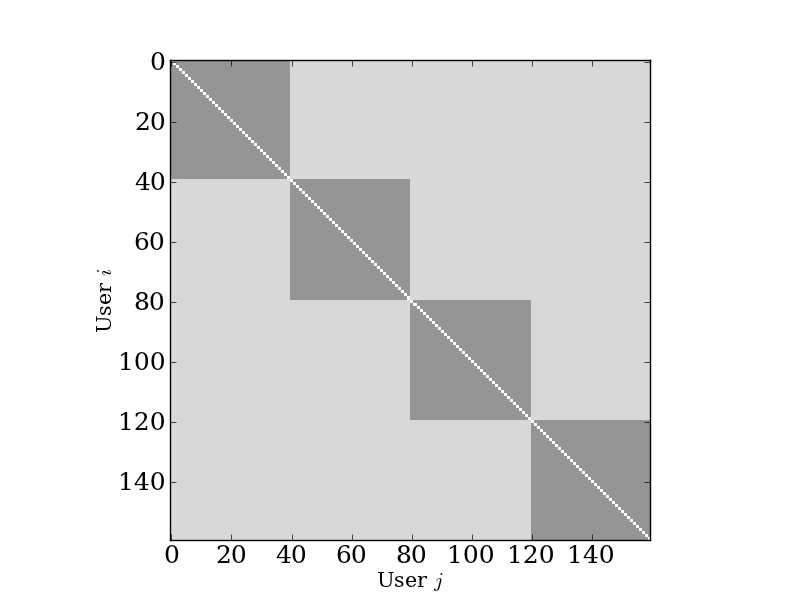
\includegraphics[width=0.75\textwidth]{Figures/prob_mat.png}
\caption{The edge probability matrix \textbf{P} for a stochastic block model with four communities each with 40 members.}
\label{Fig-SBM}
\end{figure}

\begin{figure}[h!]
  \centering
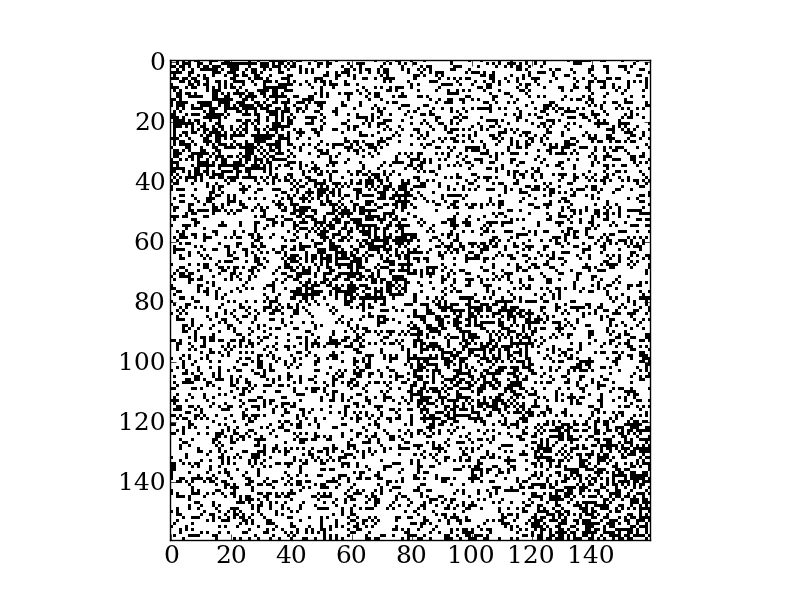
\includegraphics[width=0.75\textwidth]{Figures/adj_mat.png}
\caption{The (undirected) adjacency matrix $\mathbf{A}$ from a realization of the stochastic block model specified by the edge probability matrix \textbf{P} from Figure~\ref{Fig-SBM}.}
\label{Fig-SBM_Realization}
\end{figure}

\subsubsection{Coupled Bernoulli Process}

Previous work~\cite{ver2012information} has considered modeling users on Twitter as coupled Poisson processes. In this model, the users are embedded in a directed network, with each vertex in the graph corresponding to a user and each directed edge indicating the presence of `influence' of the initiating user on the terminal user. Influence was modeled as follows: after a user $u$ tweets, the user exerts an influence on its directed neighbors by increasing the instantaneous rate of their associated Poisson process for some interval of time. The authors of~\cite{ver2012information} took the coupling term to decay as a reciprocal power of the time since the tweet occurred.

In this work, we consider a modified version of this model. (\textbf{Mention connections to (directed) Susceptible-Infected-Susceptible type models?}) First, since communication on digital social networks such as Twitter occur in discrete time, we explicitly model each user as a \emph{Bernoulli} process, the discrete-time analog of a Poisson process. Second, in this initial work, we only consider an influence to occur over a single time delay. This corresponds to a choice of time scale. Thus, at a given time instant $t$, the probability of a particular user tweeting, given the entire past behavior of all of the users is
\begin{align}
	P(X(t, v) = 1 | \mathbf{X}(t-1), \mathbf{X}(t-2), \ldots) &= P(X(t,v) = 1 | \{ X(t-1, u) : u \in \mathcal{N}(v)\})\\
	&=\min \left\{p_{v} + \sum_{u \in \mathcal{N}(v)} \iota_{uv} 1[X(t-1, u) = 1], 1\right\} \label{Eq-Bernoulli_Model}
\end{align}
where $\mathcal{N}(v)$ denotes the directed neighbors of $v$ (those users in the network with directed edges from themselves to $v$), and $\iota_{uv}$ denotes the influence of user $u$ on user $v$.

\begin{figure}[h!]
  \centering
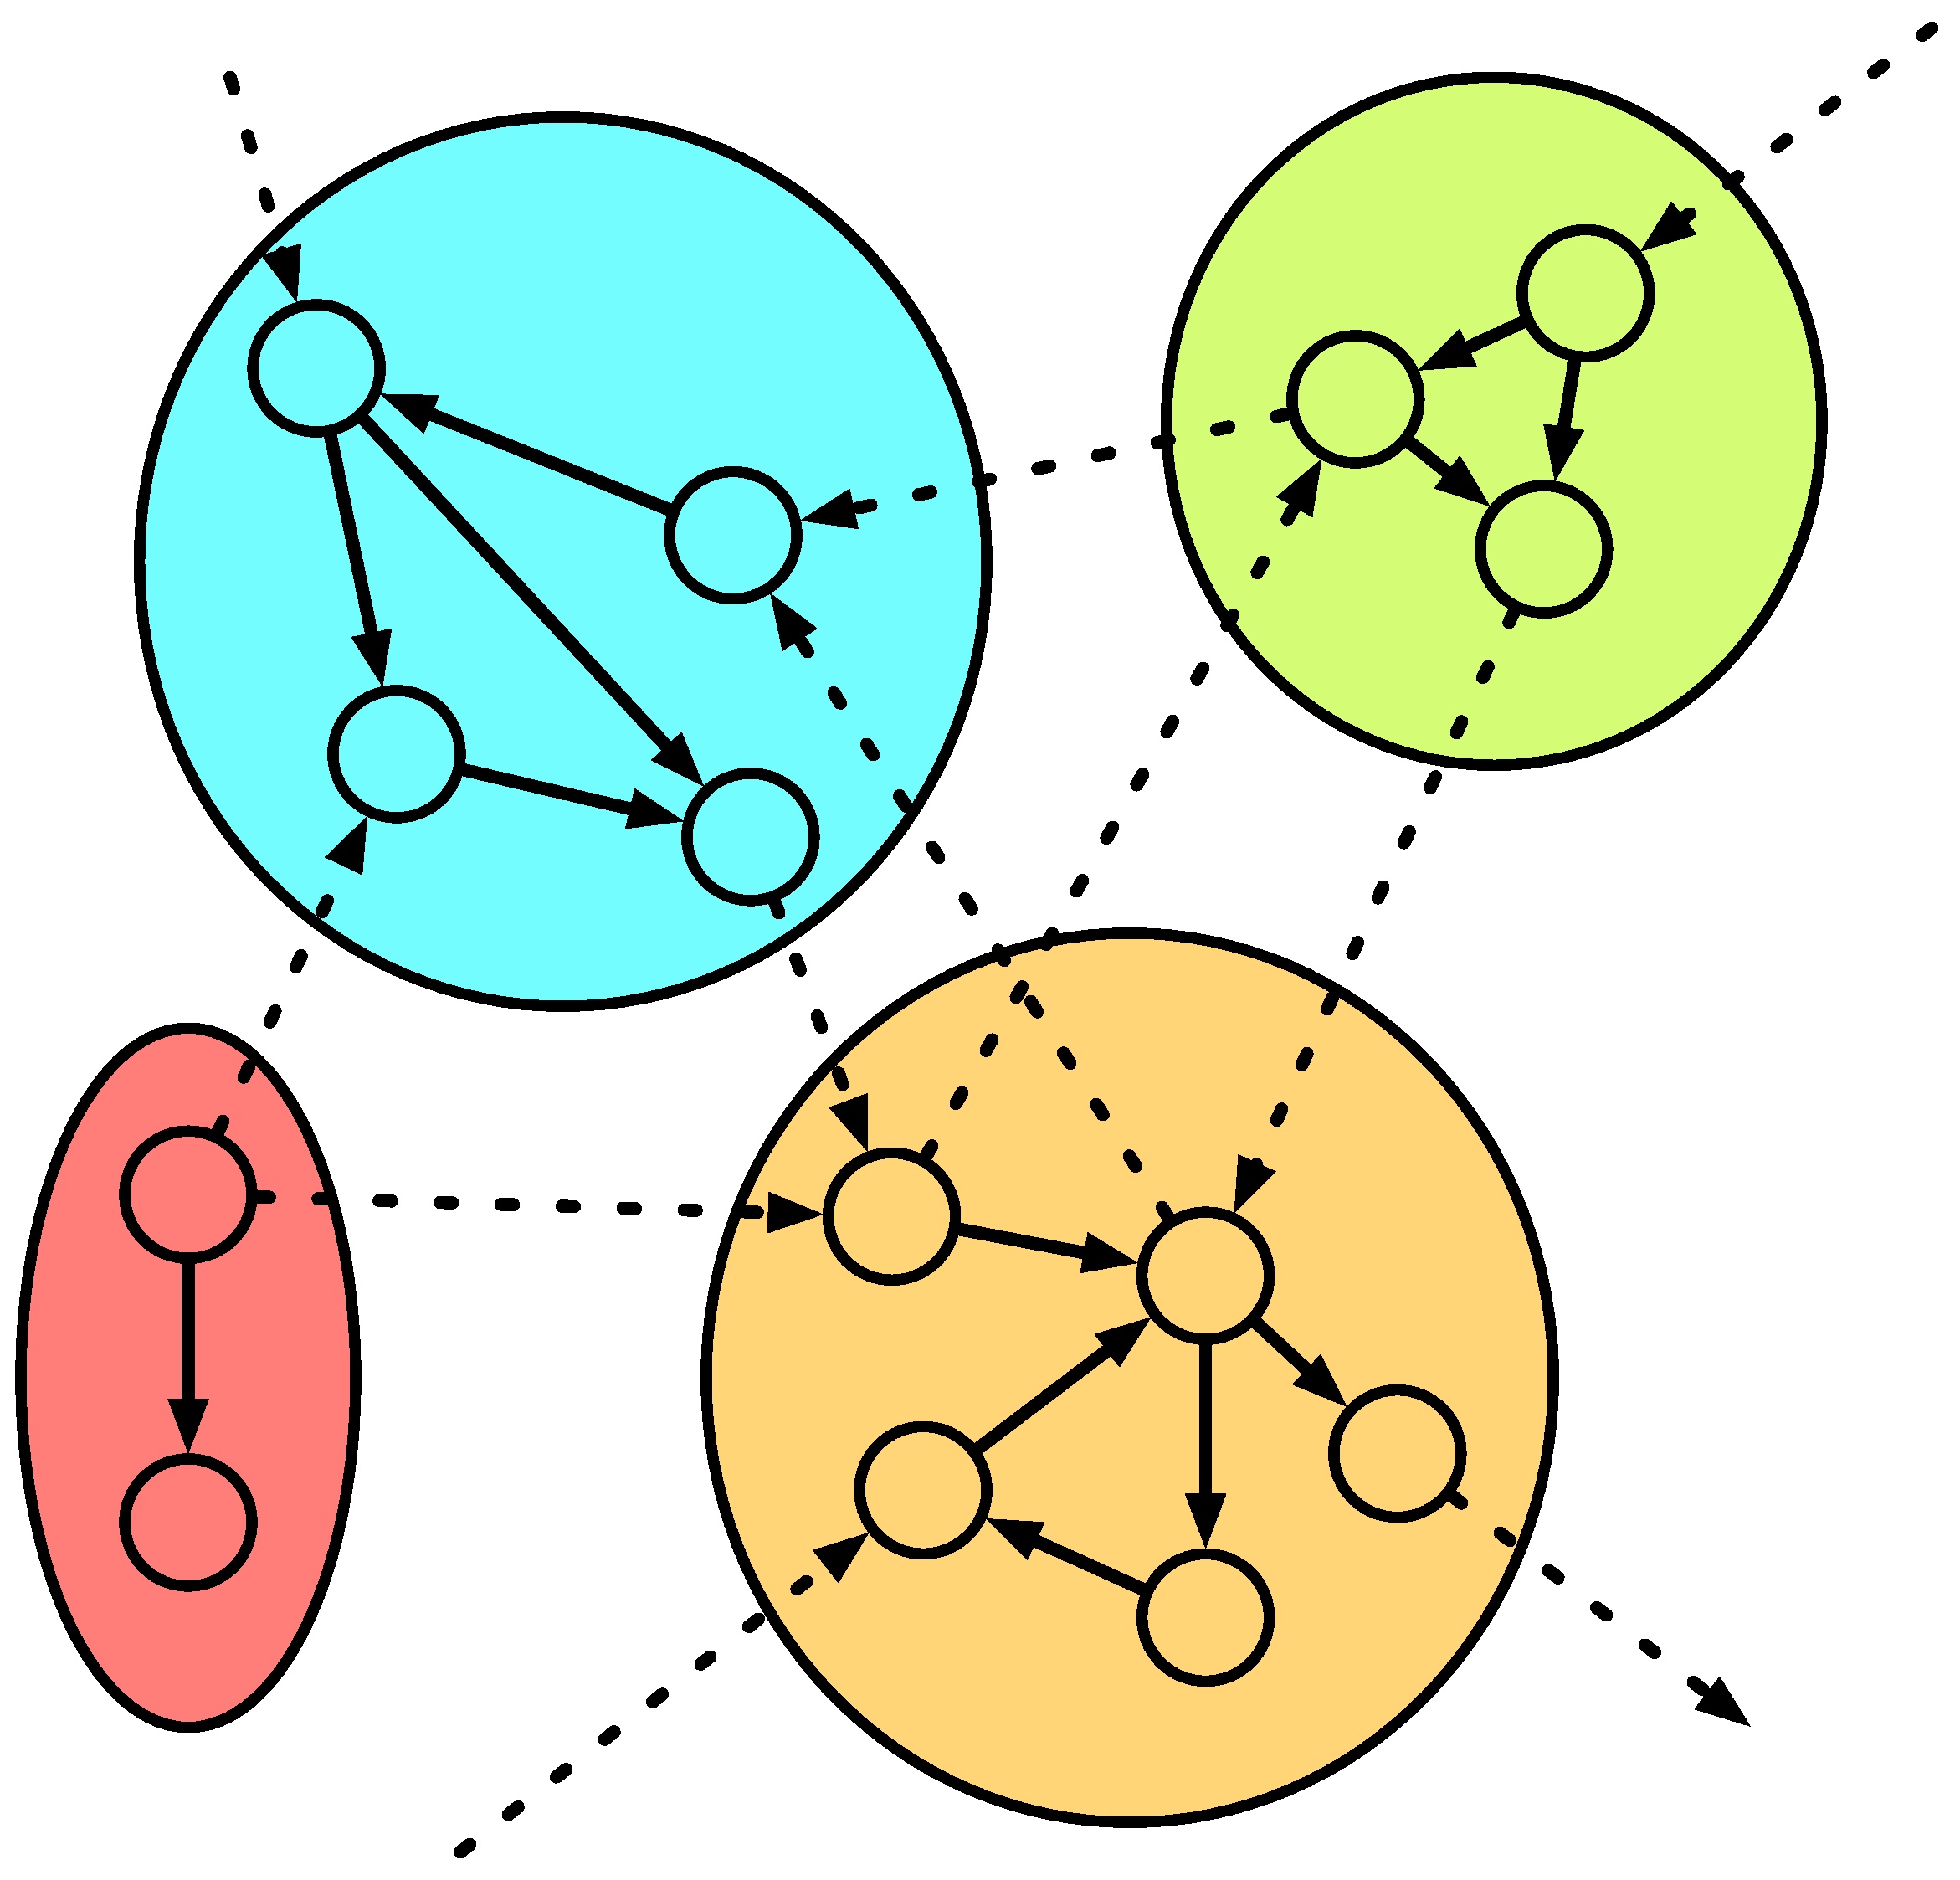
\includegraphics[width=0.3\textwidth]{Figures/Communities.eps} \hspace{1 in}
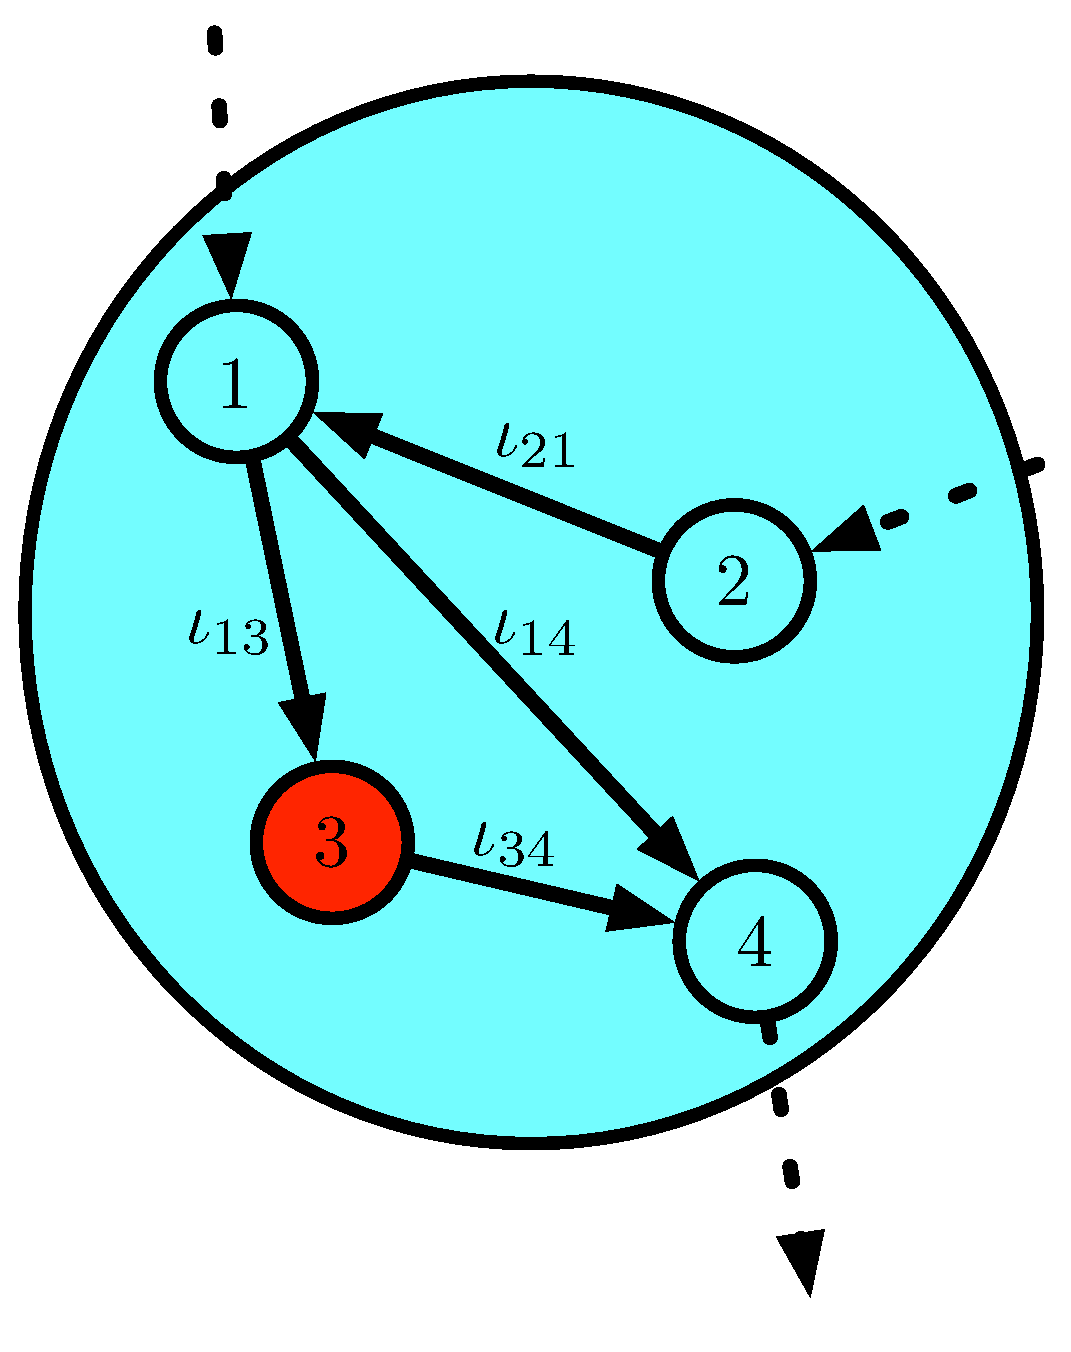
\includegraphics[width=0.3\textwidth]{Figures/Toy2.eps}
\caption{Schematics for the coupled Bernoulli model. Left: A collection of communities defined by the dynamics of their users. Right: Focusing on the influencers of a particular user.}
\label{Fig-Toy_Bernoulli}
\end{figure}

A schematic for this model is shown in Figure~\ref{Fig-Toy_Bernoulli}. In the left schematic, each solid circle corresponds to a set of nodes in a particular dynamical / functional (\textbf{whatever word we decide to use}) community. Note that these communities may differ from the \emph{structural communities} as defined by the stochastic block model in Section \ref{Sec-SBM}. In particular, we will take $\iota_{uv}$ to be larger between two nodes $u$ and $v$ within the dynamical community than between two nodes in different dynamical communities. In the right schematic, we focus on user 3. For this user, we see that the equation determining the probability of that user tweeting at time $t$ (Equation (\ref{Eq-Bernoulli_Model})) reduces to
\begin{align}
	P(X(t, 3) = 1 | \mathbf{X}(t-1), \ldots) &= P(X(t,3) = 1 | X(t, 1)) \\
		&= \min \left\{p_{3} + \iota_{13} 1[X(t-1, 1) = 1], 1\right\}\\
		&= \text{base rate } + \text{ influence,}
\end{align}
a base probability plus the influence of 3's directed neighbors.

\subsubsection{Choice of Parameters for Toy Model}

For the results presented in this paper, we took $p_{\text{in}} = p_{\text{out}} = p = \ldots$ (\textbf{not in the code... but I can figure it out from the sampled adjacency matrix}). Thus, any `structural' communities are spurious. For each edge generated by the stochastic block model, the direction of the edge was chosen at random. We took $\iota_{\text{in}} = \frac{0.7}{4}$ and $\iota_{\text{out}} = \frac{0.07}{4}$. Thus, the influence of users within a dynamical community is ten times the influence of users outside the dynamical community. The value for $\iota_{\text{in}}$ was chosen to be below a critical value $\iota^{*}_{\text{in}}$ (dependent on $p$) that lead the users in each community to constantly tweet.

\subsection{Twitter Dataset}

The data consists of the Twitter statuses of 12,043 users over a 49 day period. The users are embedded in a 15,000 node network collected by performing a breadth-first expansion from a seed user. Once the seed user was chosen, the network was expanded to include his/her followers, only including users considered to be active (users who tweeted at least once per day over the past one hundred tweets). Network collection continued in this fashion by considering the active followers of the active followers of the seed, etc.

The statuses of each user were transformed into a binary time series using their time stamp as follows. For each user $u$, we consider only the relative times of their tweets with respect to a reference time. Denote these times by $\{ \tau^{u}_{j}\}_{j = 1}^{n_{u}}$. Let the reference start time be $t_{0}$ and the coarsening amount be $\Delta t$. From the tweet times, we can generate a binary time series $\{ X(i, u)\}_{i = 1}^{T}$, where
\begin{align}
	X(i, u) = \left\{ \begin{array}{cl}
		1 &: \text{$ \exists \tau^{u}_{j} \in [t_{0} + (i - 1) \Delta t, t_{0} + i \Delta t)$} \\
		0 &: \text{ otherwise}
	\end{array}\right. .
\end{align}
In words, $X(i, u)$ is 1 if user $u$ tweeted at least once in the time interval $[t_{0} + (i - 1) \Delta t, t_{0} + i \Delta t)$, and 0 otherwise. Because the recorded time of tweets is restricted to a 1-second resolution, a natural choice for $\Delta t$ is 1 second. However, computing mutual information between second-resolution tweet series would neglect medium- to long-range influences between individuals. Thus, we generally take $\Delta t$ to be on the order of minutes.

In this paper, only tweets made between 7 AM and 10 PM (EST) were considered. For any second during this time window, a user either tweets, or does not. Thus, each day can be considered as a binary time series of length 57,600, with a 1 at a timepoint if the user tweets, and a 0 otherwise.

\section{Results}

\subsection{Community Detection --- Structural vs. Dynamical Links}

In order to test our hypothesis we ran a community detection algorithm on the two networks under analysis: the one produced by the toy model and the Twitter one. 
We used the algorithm developed by Blondel at al. \cite{blondel2008fast}, which is found to be one of the best algorithms for community detection based on modularity 
optimization, as shown by Fortunato in his review of communities detection methods\cite{fortunato2010community}. 
The algorithm works in two phases: in the first one the modularity is optimized by allowing only local changes of communities, 
and in the second one the found communities are aggregated in order to build a new network of communities. 
These two phases are repeated iteratively until no increase of modularity is possible.
In the future we plan to expand the analysis by using also other algorithms, such as Infomap\cite{rosvall2010mapping}, and compare the obtained results.
The analysis was carried out in two steps: first we applied the algorithm to the binary unweighted network, considering in this way only the \textit{structural}
relationships between the nodes. These are given, in the case of the real data, by looking at who is \textit{following} who on Twitter, which is an
explicitly declared relationship. The limitation of this method is that most Twitter users follow a very large number of people, but in practice they
see and share only the tweets belonging to a relatively small subset of the users they follow. Therefore the second step was to apply the algorithm 
to a weighted version of the networks, that we obtained by weighting each structural link with the value of the mutual information between the two users.
The results of this analysis are shown in Table~\ref{table_modularity}.

\begin{center}
\begin{table}[!ht]
\caption{Communities Detection Results}
\begin{tabular}{c|c|c|c|c|}
\cline{2-5}
& \multicolumn{2}{|c|}{Synthetic Network} & \multicolumn{2}{|c|}{Twitter Network} \\ \cline{2-5}
& Binary & Weighted & Binary & Weighted \\ \cline{1-5}
\multicolumn{1}{ |c| }{Number of Detected Communities} & 8 & 4 & 26 & 37 \\ \cline{1-5}
\multicolumn{1}{ |c| }{Optimal Modularity Value} & 0.264 & 0.625 & 0.260 & 0.404 \\ \cline{1-5}
\end{tabular}
\label{table_modularity}
\end{table}
\end{center}

We can observe a clear increase in the optimal value of modularity when we consider the weighted network, which indicates that the network has a more
defined community structure. In the case of synthetic data the value triples, whereas in the case of real data it doubles. This result shows, as we expected,
that if we weight the structural links of a network with a measure of the communication flow among the nodes, giving thus more importance to the links
between two users that actually share information and less to the links that are there but are not exploited, we can detect a finer community structure.
In particular, for what concerns the synthetic data, we can observe that in the weighted case we find exactly four communities, which is coherent to the way
the toy model was built. A visual representation of the results is given in Figure~\ref{networks_synthetic} for the synthetic data and in 
Figure~\ref{networks_twitter} for the Twitter data.

Because the
representation of the network is different (binary vs weighted),
the modularity value is not enough to say that the community
structure is different. The differing values could be due to computing the modularity with and without weighting. To test this hypothesis, we consider the actual community structure in both cases. The sizes and overlap of the largest communities are shown in Table~\ref{Tab-Community_Stats}. By just looking at the number of modules in each representation,
we can be tempted to say that the community structure is different.
However, as the next table shows, the percentage of total nodes
inside the biggest five nodes is very high. In other words, the
first five biggest modules dominates the community structure.


\begin{table}
\begin{center}
\caption{Lorem ipsum.}
	\begin{tabular}{ | r | c | c | c | c | c | c |}
		\hline
		& 1 & 2 & 3 & 4 & 5 & Total \%\\ \hline
		Binary & 1092 & 941 & 410 & 292 & 12 & 97.76 \\ \hline
		Weighted & 1098 & 938 & 220 & 293 & 140 & 95.69 \\ \hline
		Shared & 876 & 777 & 66 & 244 & 0 & 69.86\label{Tab-Community_Stats} \\ \hline
		
	\end{tabular}
	\end{center}
\end{table}

First, notice that the total size (last column) of the five biggest modules very high ($>95$ \%) as already described. Second, notice
that for the binary row we sorted the modules in decreasing order.
However, for the weighted row this is not the case (see module 3 and 4).
We relabel the weighted partition in order to maximize similarity
structure with the binary partition.

\begin{figure}[!ht]
\centering
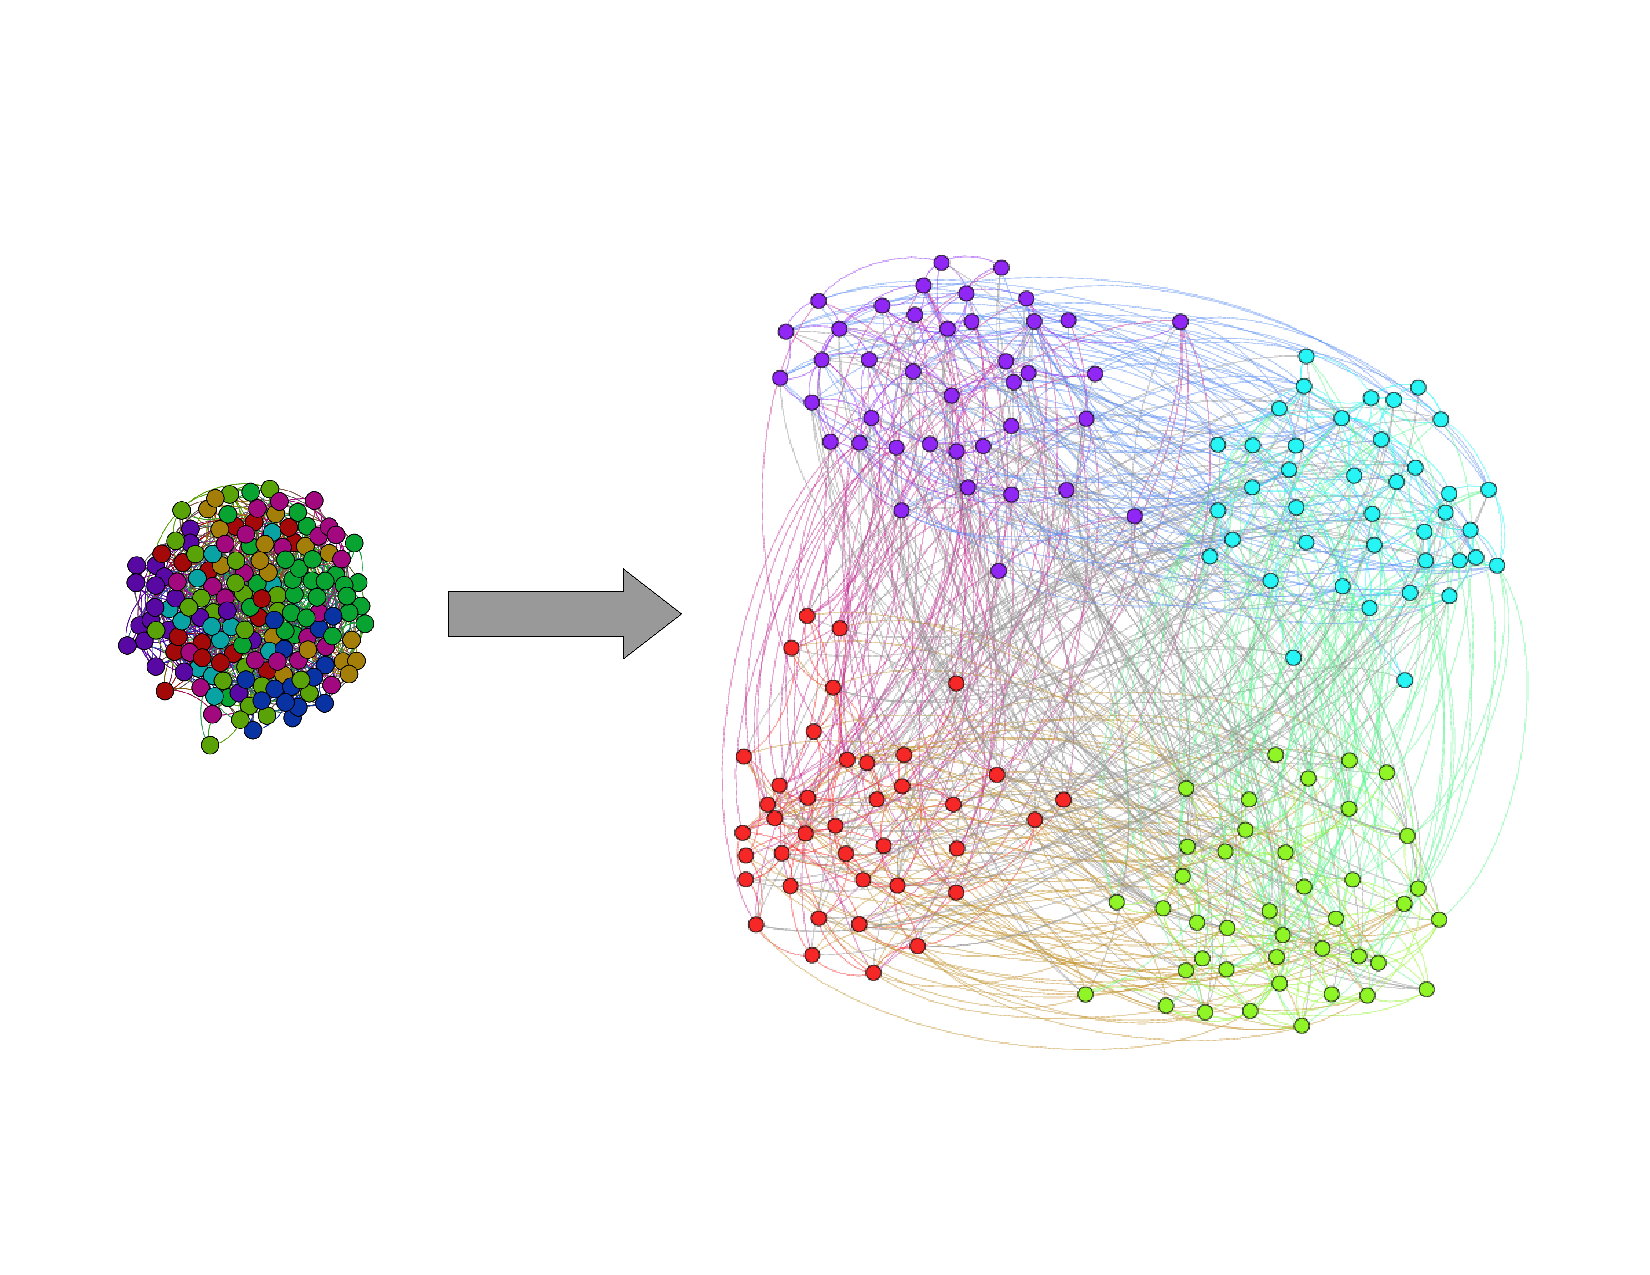
\includegraphics[width=0.72\textwidth]{Figures/synthetic_data_networks.pdf}
\caption{Visualisation of the synthetic network obtained using binary edges (left figure) and weighted ones (right figure). Node colors indicate the
community affiliation.}
\label{networks_synthetic}
\end{figure}

\begin{figure}[!ht]
\centering
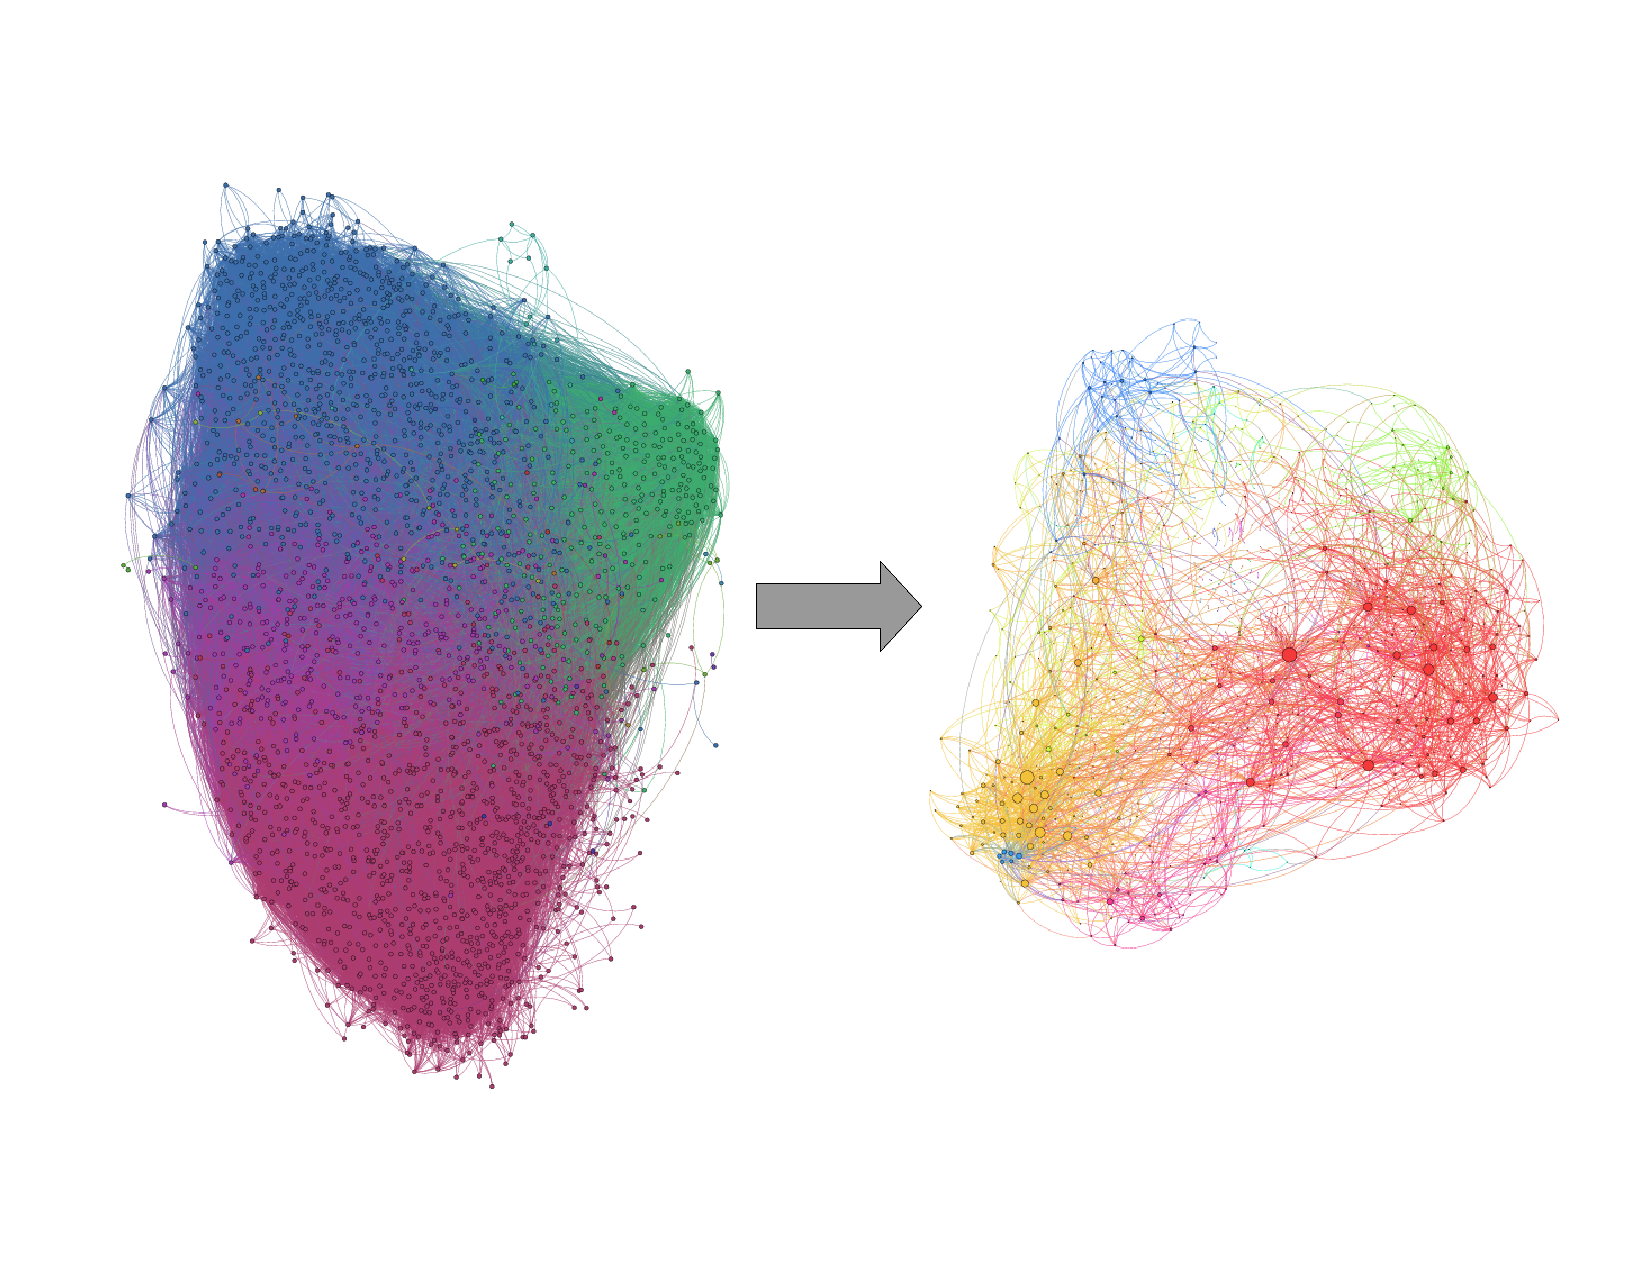
\includegraphics[width=0.72\textwidth]{Figures/twitter_data_networks.pdf}
\caption{Visualisation of the Twitter network obtained using binary edges (left figure) and weighted ones (right figure). Node colors indicate the
community affiliation.}
\label{networks_twitter}
\end{figure}

\subsection{Community Detection Across Time}

Figure \ref{fig.time.modular} represent the modularity across the
seven different weeks for a single combination of parameters. This Figure shows, that in essence, the
structure does not vary across time. This fact tell us that
for this data it may be better to just evaluate the modularity
of a single snapshot across the entire seven weeks. 

\begin{figure}
	\centering
	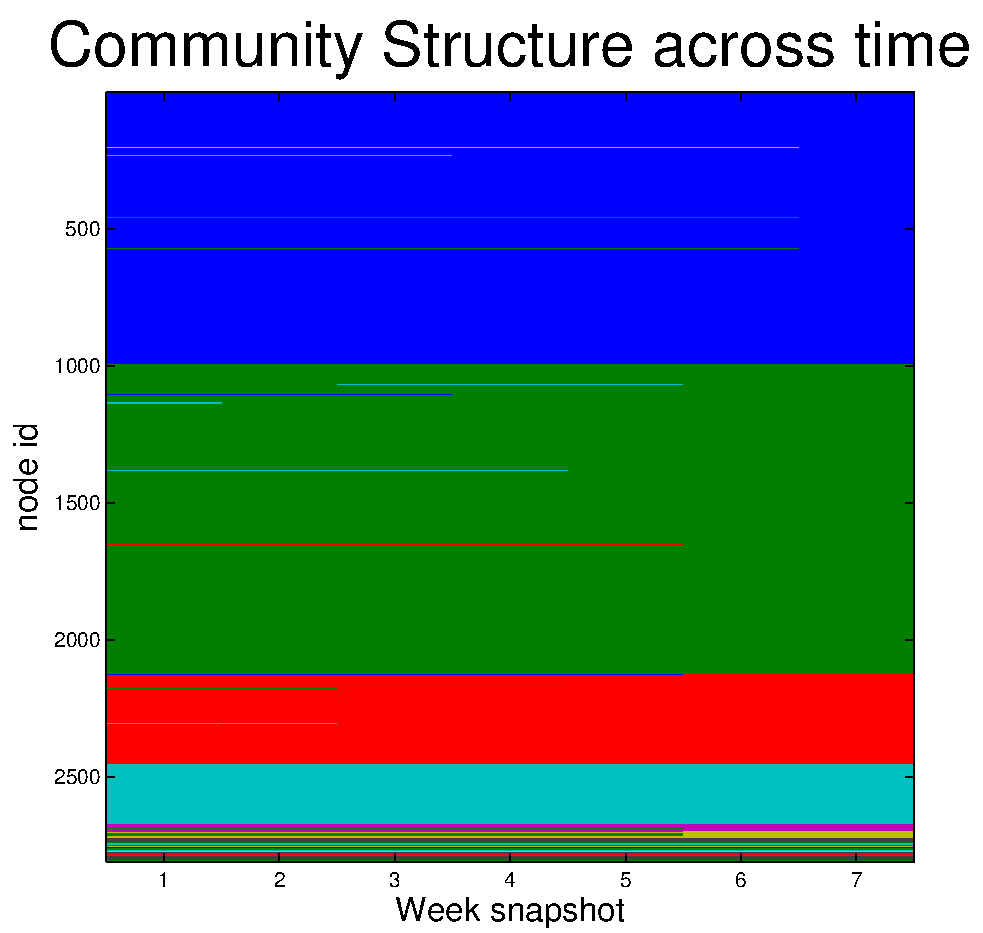
\includegraphics[width=0.87\textwidth]{Figures/modularity_time}
	\caption{Modularity across time with parameters
		$\gamma_s$ = 1 for all $s$ and $C_{jrs} = \omega=0.25$ for
		all $j,s,r$.
		 Different colors represent
		the module id to which each node (rows in this figure)
		belong to. We can observe, that the structure is dominated
		by the existence of four big modules plus a lot of small
		size modules (bottom of the Figure). Further, the modularity
		structure remains almost constant across time in the sense
		that only a very small number of nodes (represented as colored
		lines inside the big modules) switch to other modules as
		time develops.}
	\label{fig.time.modular}
\end{figure}

\section{Discussion}

Lorem ipsum.

\section{Conclusions and Future Work}

Lorem ipsum.

\bibliographystyle{plain}
\bibliography{references}

\end{document}